\documentclass[11pt]{article}
\usepackage{amssymb,amsmath}
\usepackage{graphicx} 

\title{Splotch on GPUs Using the CUDA Paradigm}
%\author{M. Rivi, C. Gheller, M.Krokos}
\author{.........}

\begin{document}
\maketitle

\section{Introduction}
\label{sec:intro}

The management and analysis of modern, large-scale datasets generated by scientific experiments, e.g. through physical observations \cite{} or numerical simulations \cite{}, can be very challenging due to continuously increasing sizes and complexity. Traditional data mining and analysis methods often rely on computationally complex
algorithms \cite{} which can be very expensive if employed for 
large-scale datasets \cite{}. Visual exploration and discovery can then represent invaluable tools, e.g. by providing scientists with prompt and intuitive insights enabling them to identify interesting characteristics and thus define regions of interest within which
to apply time-consuming methods. Additionally, they can be a very effective way in discovering and understanding correlations in data patterns, or in identifying unexpected behaviours, thus saving valuable resources, e.g. by terminating promptly on going numerical simulations producing unreliable results. Visual exploration and discovery tools can also provide effective means for communicating scientific results not only to researchers \cite{} but also to members of the general public \cite{}.

There is a long tradition within astrophysical communities in developing and deploying visual discovery tools for large-scale datasets represented by images, complex surveys, data cubes or N-body simulations. Consequently astrophysics represents an ideal discipline for exploiting High Performance Computing (HPC) devices, e.g. large multi-core and multi-node systems, providing all necessary resources for coping with large-scale datasets, e.g. computational power, large memory sizes, sufficient storage capacities and fast network speeds. A recent example is given by Hassan et al. (see related works and references in \cite{2012ASPC..461...45H}), who focus on forthcoming generations of radio surveys (ASKAP and SKA \cite{}), which are expected to produce very large datasets. Visual tools play a crucial role in exploring data cubes through a mesh-based volume rendering approach boosted by the efficient usage of GPUs. A further example, is given by Fraedrich et al. \cite{Fraedrich:2009:TMV}, who
investigated scalability in visualizing large-scale particle-based cosmological 
simulations focusing on the Millennium run \cite{millennium}, and presented methods to reduce the associated limitations on PC architectures based on levels-of-detail.
Recently Kaheler et al. \cite{2012arXiv1208.3206K} presented an algorithm specifically designed for N-body simulations. Their approach is based on a tetrahedral tessellation of the computational domain with mesh vertices defined by the simulation's dark matter particle positions and offers several GPU-assisted rendering solutions. This article includes an excellent review of methods for effective visualisation of particle based datasets (the reader is referred to \cite{2012arXiv1208.3206K} for details).

A number of popular, open-source software packages attempt to address the challenges associated with large-scale datasets and exploitation of HPC devices, e.g. VisIt \cite{visit} and Paraview \cite{paraview}. Both are based on VTK \cite{vtk} and support a fairly large variety of data types, file formats and visual discovery solutions. They can be used either as stand alone tools (running on a user's workstation) or in a client-server configuration (deploying services remotely). Both tools support in-situ visualization allowing visualization procedures to be embedded in a simulation, thus generating images during a simulation run (i.e. no data files are required) and enabling computational steering. An application of ParaView to large-scale cosmological simulations can be found in \cite{2011ApJS..195...11W}. Neither of the these packages provides customised tools for astrophysics,  e.g. particle visualization capabilities are limited. Often the underlying computational performances and/or memory usage are not highly optimized, thus preventing effective deployment of these packages on modern, large-scale astrophysical datasets. A VTK-based open-source software package focusing on astrophysics is VisIVO \cite{}. Although its main limitation is lack of interactivity, it has been recently released in the form of a science gateway offering a web-based, workflow-enabled framework seamlessly integrating large-scale, multi-dimensional datasets and applications for processing and visualization by exploiting distributed computing infrastructures \cite{}. Advanced users are able to create, change, invoke, and monitor workflows while standard users are provided with customized web interfaces hiding all underlying technical aspects. Tipsy \cite{tipsyurl} and Splash \cite{splash} are further examples of software packages specifically designed for particle-based datasets. Applicability of these packages to large-scale datasets is limited as they operate in stand-alone mode without any support for HPC resources.

This paper concentrates on {\it Splotch} \cite{2008NJPh...10l5006D} which is a ray-casting algorithm for effectively visualizing large-scale, particle-based numerical simulations. Very high-quality visualisations can be generated by Splotch for modern large-scale cosmological simulations, e.g. the Millennium trilogy \cite{millennium}, the Horizon and MareNostrum runs \cite{horizon} or the DEUS simulation \cite{deus}. The underlying models in these simulations typically reproduce the evolution of a representative fraction of the universe by means of hundreds of billions of fluid elements (described as particles) and interacting with each other through gravitational forces. The typical size of a fixed time output (or {\it snapshot}) employed by Splotch can range from several hundreds of GBs to a number of tens of TBs recording ID, position and velocity of particles together with additional properties, e.g. local smoothing length, density and velocity dispersion. Although developed for numerical simulations, Splotch has being successfully used 
also in other contexts, e.g. visualizing real galaxy systems \cite{}.

%, whose 3D shape is carefully modeled
%according to observational data. Here, more than the data size, the driver is
%the quality and the level of details of the final images,
%that have to reproduce the full details and the
%spectacular features of astronomical objects. Furthermore,
%it was adopted also for the visualization of meshed based astrophysical simulations
%(although the same high quality cannot be achieved unless extremely high resolution
%meshes are provided).

The original Splotch algorithm has been optimized in terms of memory usage and exploitation of standard HPC architectures, e.g. multi-core processors and multi-node supercomputing systems by adopting the MPI paradigm \cite{jin:high-performance} and OpenMP (see Appendix). However nowadays HPC systems are increasingly populated with GPUs employed not just as graphic accelerators but also as computational co-processors providing outstanding performances with power consumption being comparable to standard CPUs \cite{}. On suitable classes of algorithms, GPUs can ensure speed-up factors of about an order of magnitude with respect to that of standard multicore CPU \cite{}. Supercomputers are thus increasingly equipped with several hundreds of GPUs that can overlap their computing capability with that of CPUs, minimising considerably overall times-to-solution of high-end scientific problems.

This paper discusses the issues we faced in designing and implementing a new version of Splotch using the CUDA paradigm to fully exploit modern HPC infrastructures. The main issue was optimizing rendering of variable radius particles, dependent both on their intrinsic size and on the point of view, posing several problems for the GPU computation in terms of race conditions and workload balancing. A preliminary investigation as reported in \cite{jin:high-performance} had to be redesigned from the ground up to avoid data transfers during GPU computation. We have deployed the Thrust library \cite{thrusturl} and designed a number of optimized solutions for rendering particles according to a new classification strategy. Our approach accelerates the original Splotch by a factor of 5 and considering exploitation of OpenMP this acceleration can reach a factor of 8.  This improved performance is achieved without affecting the performance features of the original Splotch - linear scalability on the number of particles and image sizes. Section 2 is a short description of the Splotch algorithmic approach. Background on GPU architectures and a performance model that guided our re-designing of Splotch are discussed in section 3. Our implementation is presented in section 4 in which we describe our strategy on how to classify particles and rendering them accordingly. Section 5 presents our reference datasets for benchmarking and discusses performance results including scalability related to sizes of datasets and smoothing radius. Section 6 presents conclusions and pointers to future developments.

\section{Splotch Overview}
\label{sec:overview}

Splotch generates very high-quality images through a customised ray-casting approach. Large-scale datasets are supported by exploiting HPC architectures by means of an effective mix of OpenMP / MPI parallel programming paradigms.  
%through an optimal usage of memory, i.e. no data replicas or unnecessary allocations, 64 bits support and usage of shared and distributed memories. The current implementation of Splotch \cite{} adheres to a simple software engineering design allowing for easy extensions, e.g. incorporating new data readers. 
The implementation of Splotch is self-contained with no dependencies from external libraries (apart of course from those needed for parallelism and to support specific file formats, e.g. HDF5 \cite{hdf5}). The code is pure C++ and compilation is straightforward through suitable makefile scripts. The operational scenario is described in detail in \cite{2008NJPh...10l5006D}. To aid the presentation in this paper the main stages of Splotch as summarised as below:
\begin{itemize}
\item
{\it Data Loading} - Several readers are available supporting different formats. As a minimum ($x$, $y$, $z$) scalars are required representing the positions of particles in cartesian or any other (user-defined) customized coordinate systems.
\item
{\it Rasterization and Processing} - Firstly, normalisation together with other necessary 
calculations (e.g. logarithms of processed quantities) are performed. Secondly, particle 
coordinates and other geometric quantities (e.g. smoothing lengths - see below) are 
roto-translated and projected according to camera settings. At the end of this
stage particle coordinates are calculated in the image reference frame. % CLAUDIO THIS PREVIOUS SENTENCE IS UNCLEAR TO THE UNFAMILIAR READER, I.E. WHAT IS THE IMAGE REFERENCE FRAME? I SUGGEST TO DELETE COMPLETELY
At this point all active 
particles (i.e. contributing to the final rendering) are identified.
For the sake of simplicity in the following sections 
this phase will be referred to as {\it Rasterization}.
\item
{\it Rendering} - The contributions of individual particles to pixels of the final 
image are calculated by solving the radiative transfer equation  \cite{1991par..book.....S}:
\begin{equation}\label{rad}
\frac{d\bf{I_{\lambda}}(x)}{dx}=(\bf{E}_p-\bf{A}_p\bf{I_{\lambda}}(x))\rho_p^{\lambda}(x),
\end{equation}
where $I_{\lambda}$ is the intensity of pixel $x$ for its three color components ($\lambda$ = R, G and B), $\rho_p^{\lambda}(x)$ is a physical quantity transported by the particle $p$ 
(e.g. temperature or density),
which contributes to the intensity of color $\lambda$ of pixel $x$, and $\bf{E}_p$ and $\bf{A}_p$
are the coefficients of radiation emission and absorption respectively. These two coefficients 
can be associated to a physical quantity transported by particle $p$.% CLAUDIO THIS PREVIOUS SENTENCE IS UNCLEAR TO THE UNFAMILIAR READER, I SUGGEST TO EITHER REPHRASE OR DELETE COMPLETELY
\end{itemize}
Equation \eqref{rad} is solved for each color component using a finite differences 
approximation along a line of sight originating from each pixel on the final rendering. Each 
particle contributes to a pixel according to a Gaussian distribution:
\begin{equation}\label{smooth}
\rho_p^{\lambda}(x)=\rho_{0,p}^{\lambda}\exp(-r^2/\sigma_p^2),
\end{equation}
where $\rho_{0,p}^{\lambda}$ comes from the input simulation, 
$r$ is the distance of the particle $p$ from the pixel and 
$\sigma_p$ is a smoothing length deployed for modelling the particle size. 
Although individual particles contribute to all pixels of the rendered images, 
for practical purposes it is handy to use a compact support of this
Gaussian distribution. The distribution is considered to be zero at a given
distance $\chi\cdot\sigma_p$, where $\chi$ is a suitably-defined multiplicative factor, so that any rays passing at distances larger than $\chi\cdot\sigma_p$ are completely unaffected by $\rho_p$.

The RGB components can be defined by exploiting different physical quantities. For instance, colors 
can be associated to the three components of the velocity field $\bf v$, so that 
$\rho_p^{R}=v_x$, $\rho_p^{G}=v_y$ and $\rho_p^{B}=v_z$. Conversely, a scalar quantity, such as mass density or temperatures, can be mapped
to the RGB components via colour look-up tables (or palettes). The emission and absorption coefficients have in general different values. However for parallel implementations of Splotch $\bf{E}_p=\bf{A}_p$ is deployed, so that final renderings are independent of integration order of particles. This is not a severe restriction, it allows to simplify parallel implementations of the algorithm to so as to improve performances, without affecting, in most cases, the rendering quality.% CLAUDIO THIS PREVIOUS SENTENCE IS UNCLEAR TO THE UNFAMILIAR READER, WHAT EXACTY DO WE MEAN BY SAYING THAT IN MOST CASES THE RENDERING QUALITY IS NOT AFFECTED, A REVIEWER MAY ASK IN WHICH CASES IT IS AFFECTED AND BY HOW MUCH?  WE NEED TO CLARIFY HERE IF SETTING A = E IS A SERIOUS RESTRICTION OR NOT - IN ANY CASE WE CAN SAY THAT THE ORIGINAL SPLOTCH HAS A = E AND WE HAVE JUST OPTIMISED THAT FORM OF SPLOTCH BY USING CUDA SO IT DOES NOT AFFECT THE WORK PRESENTED IN THIS PAPER - BUT IT HAS TO BE CLARIFIED AS EXPLAINED PREVIOUSLY.

%The parallelised Splotch implementation mixing OpenMP / MPI, together with a discussion %on the performances achieved can be found in \cite{jin:high-performance}.
%In the same figure, also the parts subject to the GPU implementation are shown, 
%anticipating the discussion of the following sections.The workflow is shown in Figure~\ref{fig:workflow}, where the parts of the algorithm parallelized
%either with MPI or with OpenMP are emphasized. 
%\begin{figure}
%\centering
%\includegraphics[scale=0.18]{images/flowsplotch.eps}
%\caption{Splotch workflow}
%\label{fig:workflow}
%\end{figure}

\section{The GPU Code}
\label{sec:gpu-code}
GPUs represent an efficient tool to improve the performance of a numerical code.
However, algorithms have to be reimplemented in order to run on such accelerators. 
Often, a complete redesign is necessary to achieve good performace and in many
cases such performance is much lower than the nominal one. Nevertheless, even in 
the case of moderate performance improvements, a GPU enabled code allows the 
user to exploit the full power of the majority of the HPC systems currently 
available, which combine usual multicore processors with multiple graphic accelerators.

Splotch has undergone such refactoring process, adopting the CUDA paradigm 
for an effective usage of the GPU. The basic steps accomplished in
the realization of the GPU code, are presented in the next sections. 

%The potential dependency of any pixel of the image from any data point,
%makes the distribution of work between GPU's cores challenging to implement
%and even harder to tune in terms both of performance and of memory requirements.
%In section XXX, we propose a simple performance model that has
%driven the implementation of the GPU enabled Splotch kernels.

\subsection{The CUDA programming model} 
\label{sec:cuda}

For the implementation of the GPU code we have adopted the CUDA 
programming model \cite{cudaurl},
that is currently the standard ``de facto'' for GPU programming.
CUDA is developed by NVIDIA, closely mapping the underlying
hardware (NVIDIA cards), leading to an optimal tuning of the performance.
The limited portability represents its main drawback, somewhat mitigated
by the diffusion of NVIDIA GPUs.
The CUDA standard offers access to highly parallelized modern GPU architectures via a simplified C/C++ or Fortran language interface. It is designed to support joint CPU/GPU execution of an application, where serial sections are performed by the CPU (host), while those which exhibit rich amount of data parallelism, are performed by the GPU (device) as CUDA kernels. The CPU and the GPU have separate memory spaces so data must be transferred from each other via PCI Express 
bus (hereafter PCI-E). 
CUDA kernels launch is asynchronous, so that the host can
 perform the following instructions of the code while the device is computing. If one of them requires the completion 
of the kernel execution, then it is necessary to call the \textit{cudaDeviceSyncrhonize}() function before executing it.
A kernel is written for a single thread and instantiated as a grid of many lightweight parallel threads, organized into blocks of the same size. A thread is an independent element of work and maps to a hardware core (Streaming Processor - SP). A block is a 1D, 2D or 3D set of concurrently executing threads that can cooperate among themselves through barrier synchronization and ``fast'' shared memory. 
This is possible because threads belonging to the same block are executed on the same multiprocessor (SM). On the other hand
 synchronization is not possible between blocks of a grid. The limited amount of memory limits the number of 
blocks that can simultaneously reside in the same SM. Moreover when one block stalls the runtime system switch to 
a different one, hence there is no guaranteed order of execution.

Once a block is assigned to a SM, it is partitioned into 32-thread units called warps. They are scheduling units in SM:
all threads in the same warp execute the same instruction (Single-Instruction, Multiple-Thread). Hence, programmers should minimize the number of execution branches inside the same warp. It is convenient to assign a large number of warps to each SM (high occupancy), because the long waiting time of some warp instructions is hidden by executing instructions from other warps  and therefore the selection of ready warps for execution does not introduce any idle time into the execution timeline (zero-overhead thread scheduling). 

\subsection{Performance model and analysis}
\label{sec:model}

Splotch's main computational kernels are {\it Rasterization} and {\it Rendering}.
The initial data load phase, though often demanding, will not be treated
here since it is not subject to the GPU implementation. The final save image stage
is not relevant for the performance.

%The main parameters of the model are $N_{part}$, the number of particles
%to be processed, and $N_{pix}$, the number of pixels of the final image
%(in general we can consider square images with $N_{pix}=N_{pix}^2$). For 
%the Splotch's rendering kernel a third parameter must be introduced, 
%that is the average smoothing length of the particles,
%$R_s$. Its value depends both on the intrinsic "size" of the particle
%and on the position of the point of view (particle size increases getting closer to 
%the point of view).
%
%The kernels scale with these parameters as:
%\begin{align}\label{scaling}
%& N_{Norm} \propto N_{part},\\
%& N_{Geom} \propto N_{part},\\
%& N_{Color} \propto N_{part},\\
%%& N_{Sort} \propto N_{part}{\rm log}(N_{part}),\\
%& N_{Render} \propto N_{part} R_s^2,\\
%& N_{Image} \propto N_{pix}^2,
%\end{align}
%where $N_{kernel}$ is the number of operations for a given kernel.

%The Normalization, Geometry and Coloring kernels are  
%perfectly data parallel, each particle being processed independently from the others.
%Thus they are expected to fit the GPU programming model. 
%The Rendering kernel is, in general, the most computationally demanding. 
%The computational time depends in a predictable way with the number of particles and the number 
%of pixels. The most challenging dependecy, however, is from the smoothing length. 
%This dependency leads to strong changes in the computational effort and makes
%the work-load hard to balance, when this is distributed among many-processors
%systems.

In order to model the Splotch algorthm's performance, we split the different timings
required to perform the main computational steps. 
The Splotch's performance can be quantified as time spent on the CPU, time spent on the GPU
and time spent to move data among different memories:
\begin{equation}\label{Ts}
T_{TOT} = T_{cpu} + T_{pci} + T_{gpu} + T_{Mgpu},
\end{equation}
where $T_{TOT}$ is the total time, 
$T_{cpu}$ is the time spent on the CPU, $T_{gpu}$ is the time
spent on the GPU for computation, $T_{pci}$ is the time needed to move data from
the CPU to GPU and back through the PCI-E bus and $T_{Mgpu}$ is the time 
spent in moving data among the global and the shared memory on the GPU.

\medskip
\noindent
{\bf Data transfers}

\noindent
Data offload to the GPU is one of the critical steps in the algorithm. 
The minimum amount of data 
to be moved to the GPU is represented by the particles information 
(coordinates, fields, smoothing length). If $S_{part}$ is the
size of a single particle (in the current implementation $S_{part}=35$ bytes) and 
$N_{part}$ is the number of particles to be processed,
$N_{part} S_{part}$ is the total amount of particle data that has to be moved to the device.
The final processed image (the result) is the only data that has to be copied back to
the CPU. Thus, in principle, only $12 N_{pix}^2$ bytes (R, G, B float values) have to be transferred at
the end of the rendering phase. Here, $N_{pix}$ is the linear resolution in pixels of the 
image (we consider square images, the generalization to rectangular images being
straightforward). 

Particles' data offload can be accomplished either in a single or in a few operations, 
depending on the data size (if it fits the available GPU memory) and/or
in order to exploit CUDA streams, which allow to overlap communication 
and computation, hiding the data transfer overhead.  
In order to implement this solution, data has to be
split in chunks and passed to the GPU one after the other, in a loop. Whilst chuncks 
are transferred, computation on previous chuncks, already stored on the GPU
memory, can be carried out. 
The data transfer time can be estimated as:
\begin{equation}\label{pci}
T_{pci} =  N_{chunks} \tau_{pci} + {N_{part} S_{part} + 12 N_{pix}^2 \over 
\mu_{pci}},
\end{equation}
where $\tau_{pci}$ is the transfer time latency and $\mu_{pci}$ is the
bus bandwidth, $N_{chunks}$ is the number 
of copy stages. 
Equation $\eqref{pci}$ shows that performance
depends linearly both on the number of particles and on the number of pixels.
In the case of large datasets we have that
$N_{part} >> N_{pix}^2$. For instance, the test case adopted
in Section~\ref{sec:results} consists in $N_{part} \sim 10^8$
and $N_{pix}^2 \sim 10^6$. In such cases, the contribution of $N_{pix}^2$
to $T_{pci}$ is negligible.

Splitting data in sub-chunks does not
cause any meaningful overhead if the copy latency is kept small, that is:
\begin{equation}
N_{chunks} < {N_{part} S_{part}\over \tau_{pci}\mu_{pci}}.
\end{equation}
For instance, if $N_{part}$ is $O(10^8)$, $N_{chunks}$ can be up to $10^5$ before
contributing to the overhead.

Equations $\eqref{pci}$ considers only the main data tranfers of
the Splotch's algorithm. However, further data tranfers may be necessary.
This aspect will be treated in Section~\ref{sec:implementation}.

\medskip
\noindent
{\bf GPU computation}

\noindent
The time spent in processing the particles on the GPU can be estimated as:
\begin{equation}
T_{gpu} = N_{op}/\nu_{GPU},
\end{equation}
where $\nu_{GPU}$ is the GPU flops/sec rate and
\begin{equation}\label{ops}
N_{op} = N_{part}(\alpha + \gamma R_s^2) + f_{GPU},
\end{equation}
with $\alpha$ and $\gamma$ estimating the number of operation of 
the Rasterization kernel  
and of the Rendering kernel respectively. The function 
$f_{GPU}$ takes into account any GPU specific kernel (i.e. a kernel
which is not present in the original code), necessary to the GPU implementation. 

The parameter $R_s$ is the most peculiar dependency of the Splotch's rendering
algorithm. It is defined as the expectation value of the particles radii:
$R_s = <r(p)>$, where
\begin{equation}\label{radius}
r(p) = A(p){\chi \sigma_p\over S_{box}} N_{pix},
\end{equation} 
$A(p)$ being the function to tranform to image coordinates,
$\chi$ a proper factor defining the compact support size (see  
equation \eqref{smooth}) and $S_{box}$ the computational box size.
The particle radius depends both on the intrinsic properties of the particle
and on the camera position. The same particle can have a negligible size
from one point of view and it can affect the whole image from a different one.
On the other hand, particles close to each other can have different radii depending
on their intrinsic characteristics. The dependency from $r(p)$ poses 
two major problems to the GPU implementation of the rendering 
algorithm. First, two threads acting on different particles could try 
to update the same pixel (see Figure~\ref{fig:particles}).
This can cause frequent concurrent accesses to memory
which lead to wrong results. 
Second, different particles can affect a different number of pixels. Therefore, a good load balancing
between threads is hard to achieve.  
Specific solution must be designed to circumvent such difficulties 
without paying big penalties in terms of performance (as would happen, for instance,
adopting atomic updates, supported by CUDA, but too slow to be used for continuous 
updates of the pixels values).

Finally, it is interesting to stress that $T_{gpu}$ depends linearly on the number of particles. 
This feature should be preserved by the GPU implementation. In particular, the term 
$f_{GPU}$ does not have to introduce any higher order dependency from $N_{part}$. 

\begin{figure}
\centering
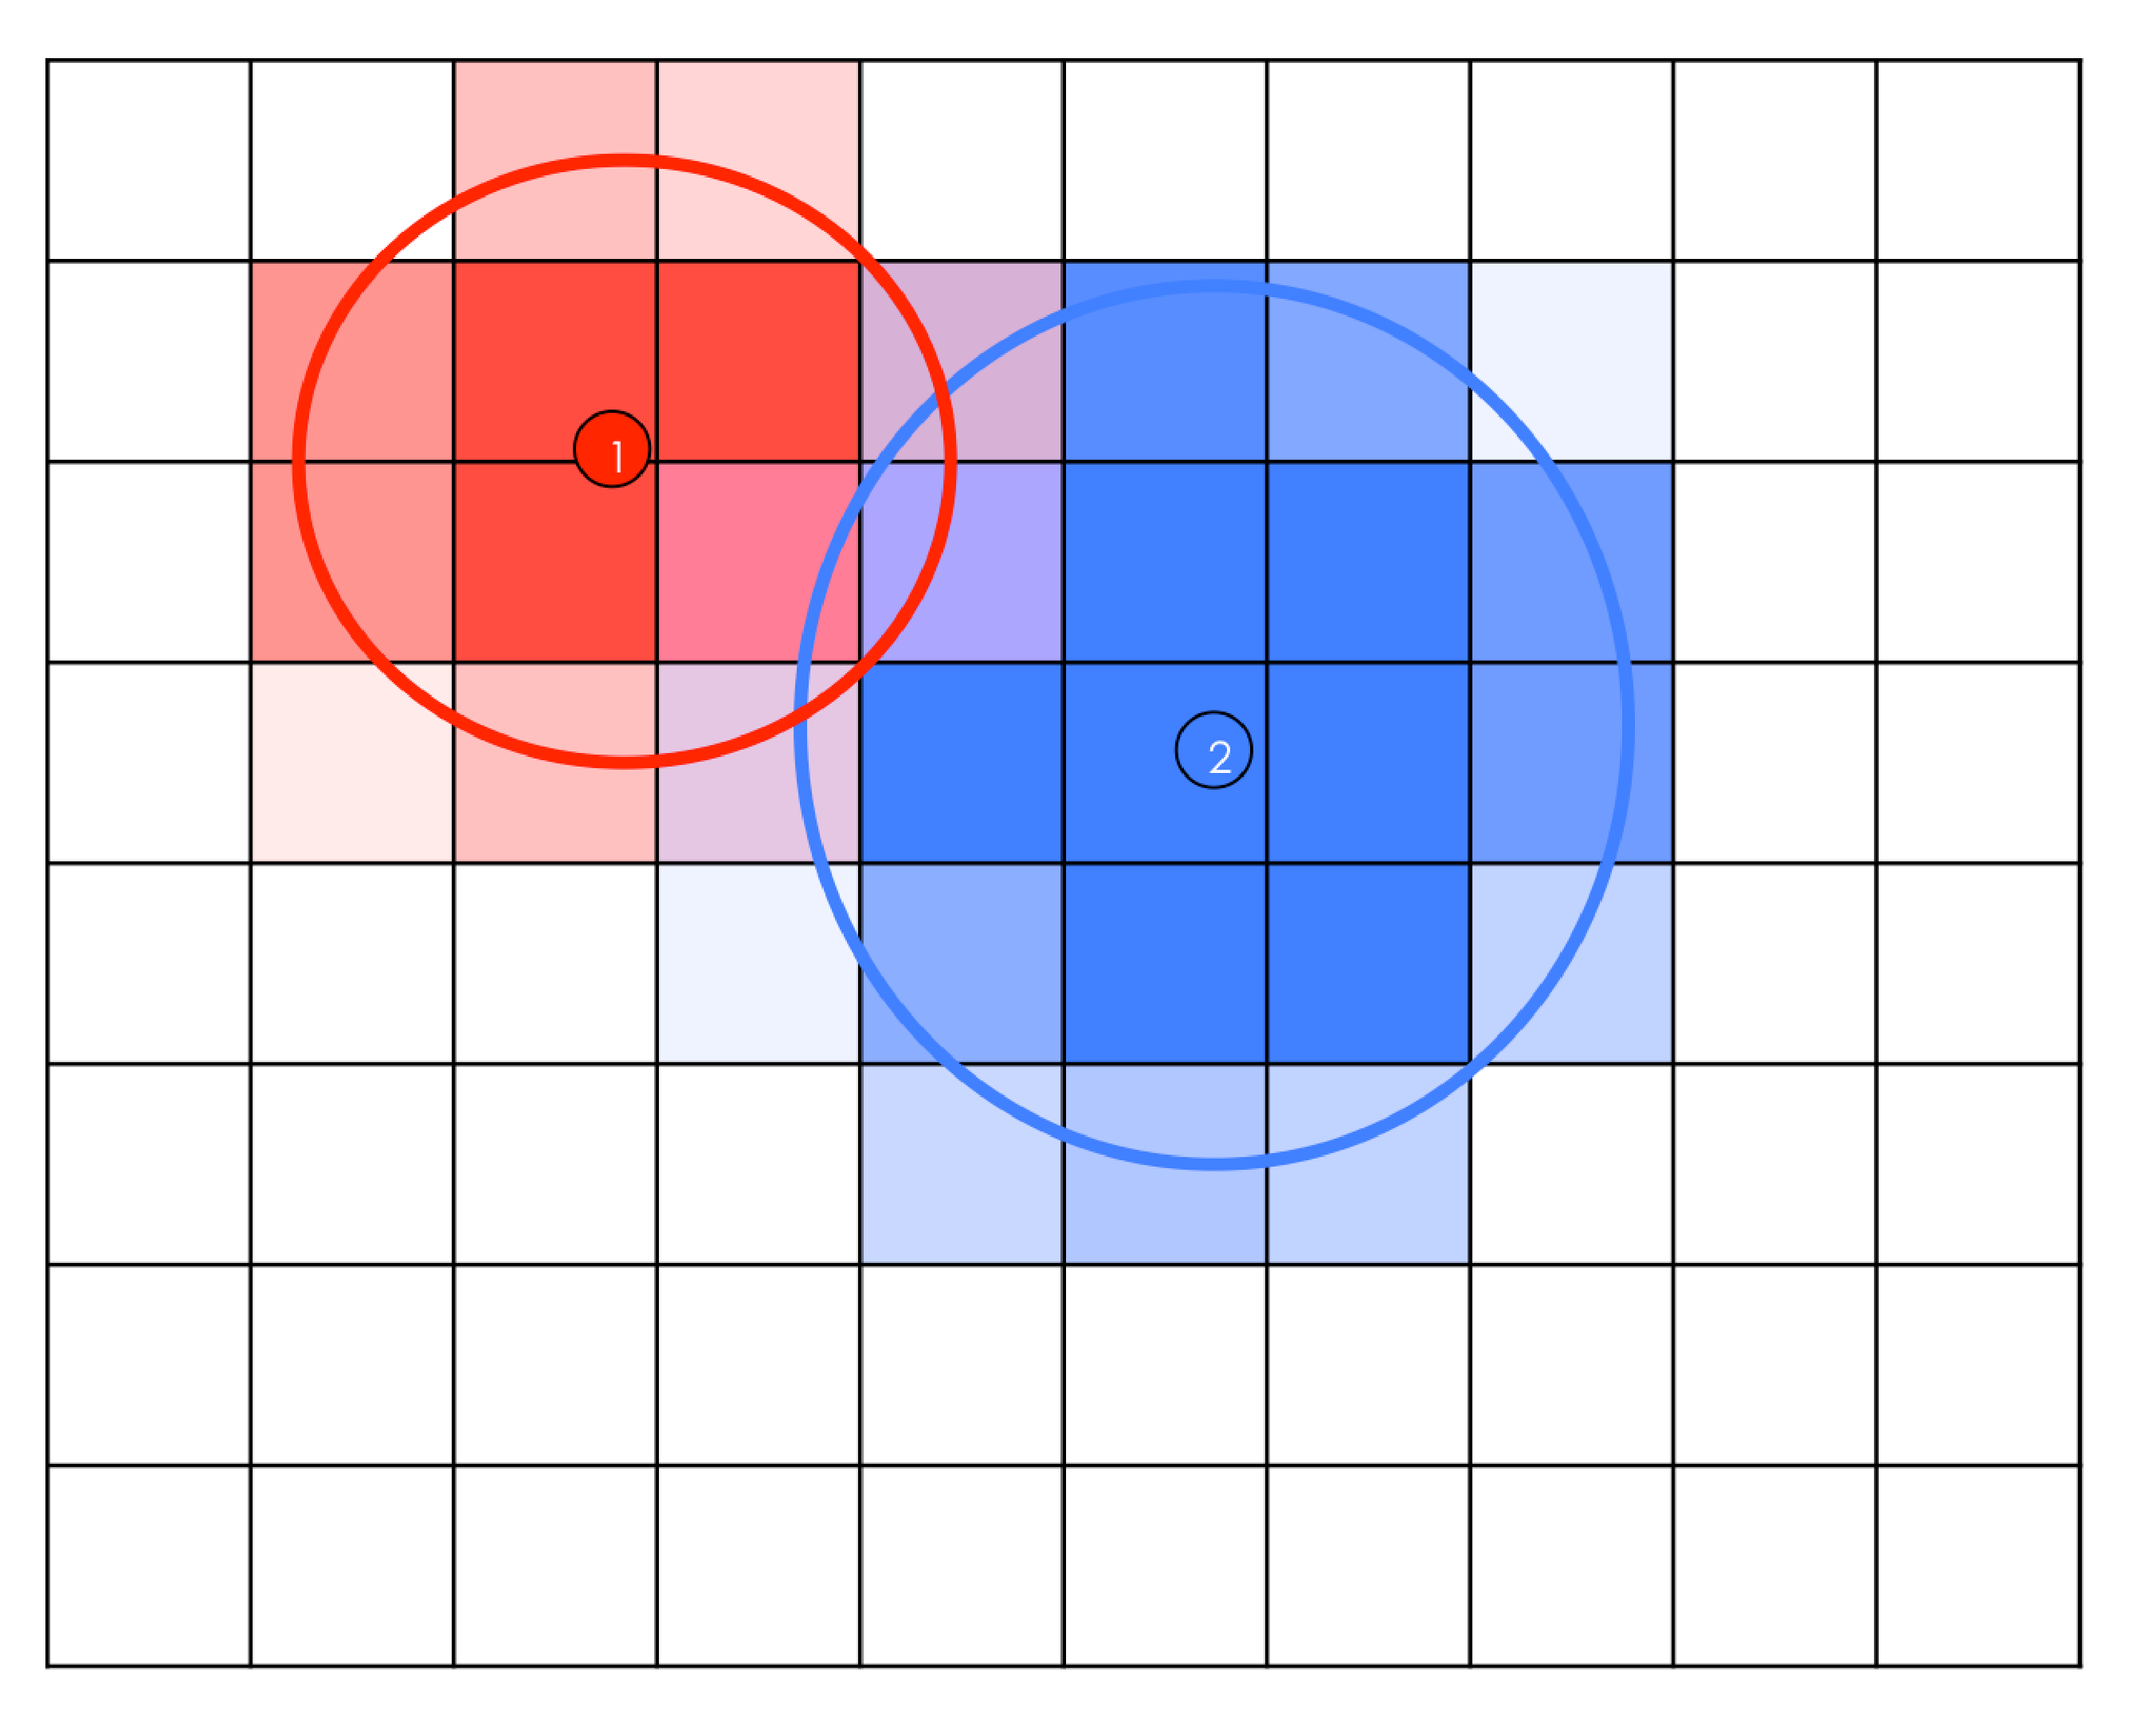
\includegraphics[scale=0.2]{images/particles.eps}
\caption{Two particles with different radii influencing the same pixels.}
\label{fig:particles}
\end{figure}


\medskip
\noindent
{\bf Memory accesses}

\noindent
Global-shared memory data transfers can be estimated 
as the number of loads from the global to the shared memory of the available 
streaming multiprocessors plus the number of stores from the shared to the global memory: 
\begin{equation}
N_{Mgpu} = (N_{load,p} + N_{store,p}) N_{part} + N_{store,pix} N_{pix}^2,
\end{equation}
where $N_{load,p}$ and $N_{store,p}$ are the number of loads and stores of the 
particles, while $N_{store,pix}$ is the number of stores of the image (no loads 
are expected, since the image is created on the GPU). 
Furthermore, memory access overhead can be estimated as $N_{Ngpu} \nu_{mem}$,
where $N_{Ngpu}$ is the total amount of memory accesses, $\nu_{mem}$
is the memory frequency. 
Hence, the time for moving data among memories is:
\begin{equation}\label{tmgpu}
T_{Mgpu} = {(N_{load,p} + N_{store,p}) N_{part} S_{part}
+ 12 N_{store,pix} N_{pix}^2\over \mu_{gpu}}
+ N_{Ngpu} \nu_{mem} + g_{GPU},
\end{equation}
where $\mu_{gpu}$ is the global memory bandwidth
and $g_{GPU}$ the time 
spent on memory accesses by the GPU specific
functions. 

Equation \eqref{tmgpu} shows that the performance related to global-shared memory 
data transfers
depends on the two parameters $N_{load,p}$ and $N_{store,p}$, that quantify the
total amount of data transferred from the global to the shared memories 
and back, whose performance depends on the memory bandwidth.
The optimal solution would be to have only a single data transfer
($N_{load,p} = 1$ and $N_{store,p} = 0$), with each thread
fully processing a different particle. This {\it one-thread-per-particle} solution guarantees
the best exploitation of the GPU architecture.
This solution, though ideal, is not practical, the main reason being the frequent race conditions
rising from threads trying to concurrently update the same pixels.
Only the Rasterization kernel is data parallel and can adopt the {\it one-thread-per-particle}
approach. Each particle, in fact, is processed independently from the others. For this kernel
$N_{load,p} = 1$ and, since processed particles
have to be copied back to the global memory to be rendered, $N_{store,p} = 1$.

The rendering part is expected to require a futher particle data load step, while no more store 
stages are necessary (particles can be ``forgotten'' after their contribution to the assigned pixels 
is calculated).

The $T_{Mgpu}$ term depends linearly on the image size. Once more, 
for large datasets, this term appears to be negligible. However, since
particles falling outside the field of view are not processed (``inactive'' particles,
see Figure~\ref{fig:fov} for an example),
depending on the camera position, the ratio between the number of active particles
and the number of pixels can substantially decrease. Therefore, 
the image related term can give a meaningful contribution to
the computing time. 

A critical term of equation \eqref{tmgpu} is represented by the memory access
latency $N_{Ngpu} \nu_{mem}$. The access to memory is slow in comparison to
the available bandwidth, so a small number of accesses, $N_{Ngpu}$, is crucial
to the performance. This can be achieved by standard caching strategies, that
however are effective only if data coalesced access (in particular data contiguity) is guaranteed. In other words,
if contiguous particle data moved to the GPU L2 cache can be reused efficiently
by the various threads. This is possible only through a global reorganization 
of the particle data. Such reorganization can however lead to an important
working and memory usage overhead.

Any further memory access specific to the GPU implementation algorithm,
must be implemented 
avoiding the introduction of eccessive overheads and preserving the overall
linear scalability with the number of particles.

\medskip
\noindent
{\bf CPU computation}

\noindent
The final contribution to equation \eqref{Ts} is $T_{cpu}$. In principle this should be negligible, 
the large part of the work being performed by the GPU. Actually, the CPU
can contribute to process part of the particles. Using
CUDA asyncronous operational mode, this work can be overlapped 
to the GPU work. 

\section{The CUDA implementation}
\label{sec:implementation}

As soon as data is loaded in the global memory of the GPU, each particle is processed 
by the Rasterization kernel. This kernel can adopt an efficient  
{\it one-thread-per-particle} approach, by which the whole computation on 
a particle (geometric tranformation, coloring etc.) is carried out
by a single thread, with no interaction with other processes.  
This approach leads to a full exploitation of the GPU architecture. 

After Rasterization, particles are ready to be rendered (Rendering kernel).
For the Rendering stage, a simple {\it one-thread-per-particle} approach
cannot be adopted (see Section~\ref{sec:model}). Furthermore, memory usage must be carefully managed.

\subsection{Rendering algorithm design}
\label{sec:design}

\begin{figure}
\centering
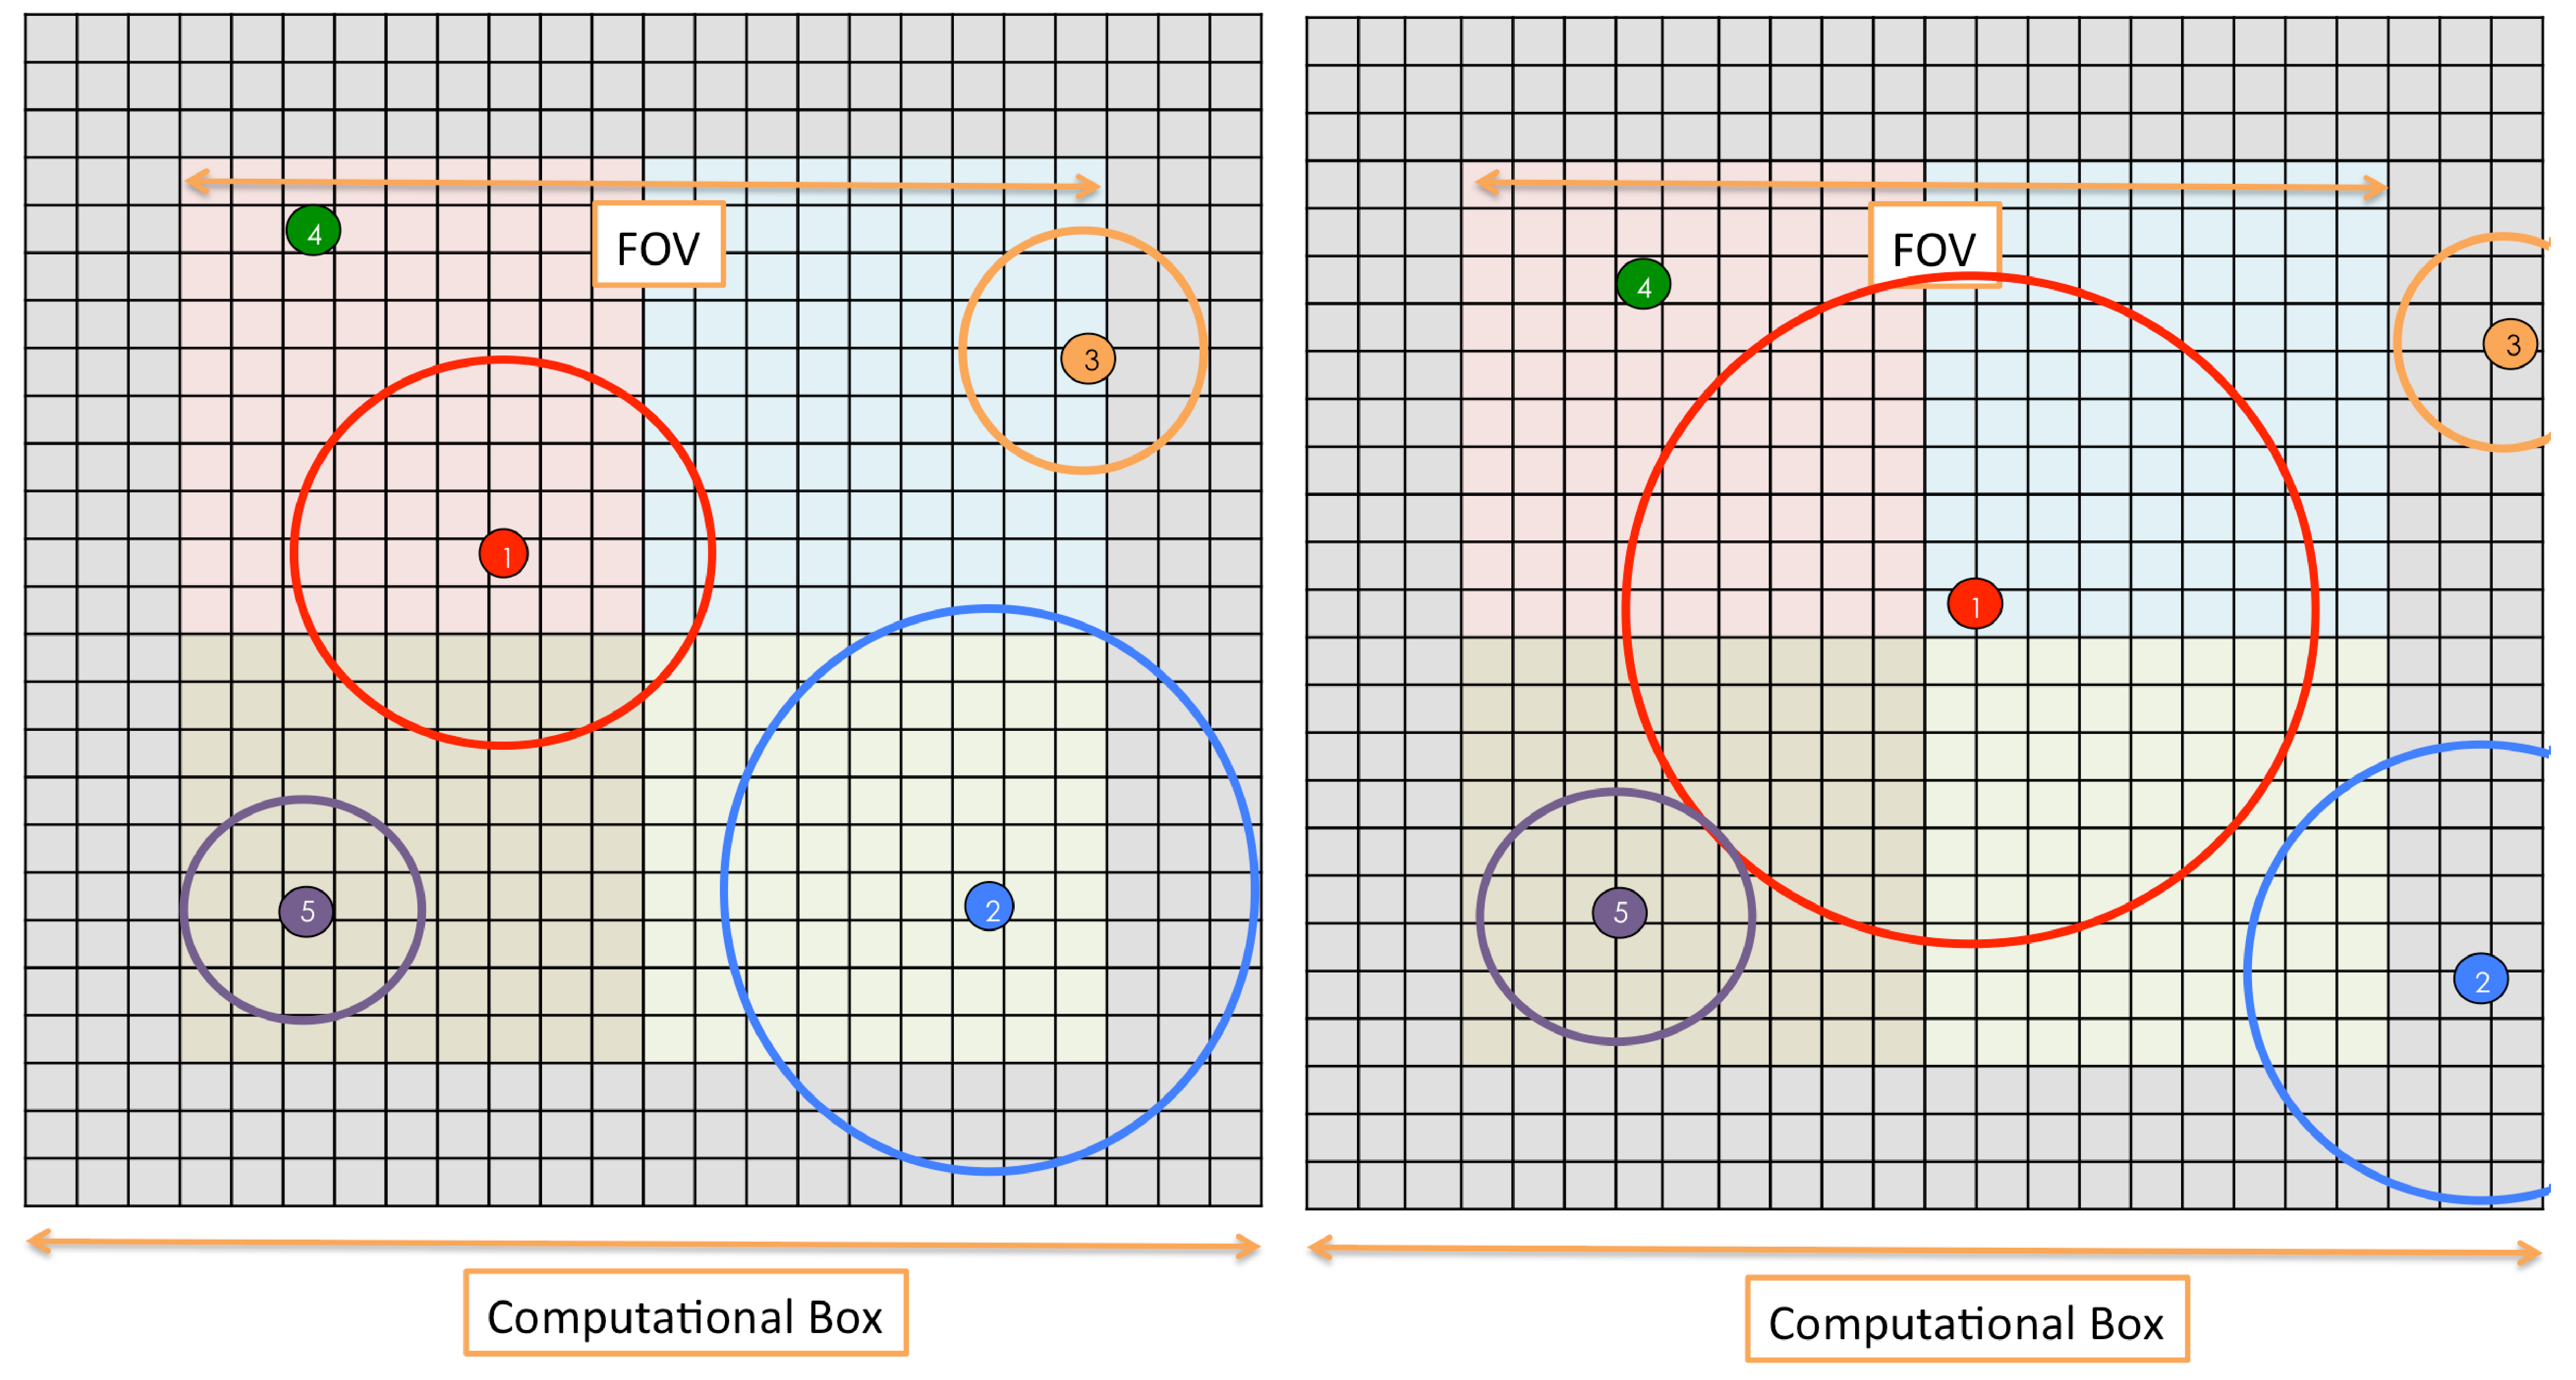
\includegraphics[scale=0.15]{images/fov.eps}
\caption{The scene with five particles from two different points of view. Different tiles are 
represented with different colors. In the first camera position
(left) all particles contributes to the image (lie in the FOV), particles 2 and 3
being classified as C2, particle 4 being C3 and particle 5 being C2. Particle 1, is classified
as C2, since it is completely contained in a {\it Btile} (in this example, it is a tile with a boundary of 3 pixels width). In the right
image the camera moved toward particle 1. All the radii change due to the new point
of view. Classification of particles 4 and 5 does not change, while particle 3 
becomes inactive (completely falling outside the FOV). Particle 2, though 
having coordinates outside the FOV, affects some pixels, hence it is still active.
Particle 1 becomes C1, since its radius exceeds the boundary width, so it exits the Btile. 
}
\label{fig:fov}
\end{figure}


On the GPU, the rendering algorithm has been designed according to the following procedure.

Particles are first classified in 3 groups according to their size:
\begin{itemize}
\item 
C1: $r(p) > r_0$
\item
C2: $0.5 < r(p) \le r_0$
\item
C3: $r(p) \le 0.5$
\end{itemize}
where $r(p)$ is the particle radius in pixels defined by equation \eqref{radius}.

Particles of different classes pose different challenges to the rendering 
algorithm and are processed with different approaches. Particles of class C3 
influence a single pixel, therefore they can be efficiently 
processed with a {\it one-thread-per-particle} approach. Setting $r_0 \sim 0.01 N_{pix}$, 
particles of class C2 can influence only small fractions of the image. If 
we divide the image in {\it tiles} of suitable size, each C2 particle can affect 
only one tile (see below for details). Finally, particles of class C1 can affect 
a large fraction of the image, spanning multiple tiles.

The particle classification is performed in the Rasterization kernel, with negligible impact
on the computing effort. Each particle is labeled
with a {\it tile index} $i(p)$ as follows:
\begin{itemize}
\item 
$i(p) = -2$, inactive particle (outside the field of view);
\item
$i(p) = -1$, if it belongs to C1 class; 
\item
$0 \le i(p) < N$, if it belongs to C2 class and its centre falls in the $i$-th tile of the image;  
\item
$i(p) = N$, if it belongs to C3 class, i.e. is point-like.
\end{itemize}
The parameter $N$ is the number of tiles the image is divided in. It is defined as
\begin{equation}
N_t = {N_{pix}^2\over t_x*t_y},   
\end{equation}
where $t_x$ and $t_y$ are the tile sides in pixels. In the code, these are input parameters 
that can be set according to the specific use case to tune the performance. As default it is set $t_x=t_y=12$ (see section~5.1 for more details). 
Figure~\ref{fig:fov} show an example of the particles classification and
how this can change with the point of view. 

After this operation, inactive and C1 particles are removed from the device memory. At this point, the remaining particles 
have to be sorted by the $i(p)$ key and the number of particles with the same index has to
be calculated. 
%At the end of this operation, all particles with the same tile index are contiguous in memory, 
%providing an optimal memory access pattern and can be easily isolated for tiles assignment and processing.
%A specific kernel has been developed to implement these operations.
The sorting operation plays a crucial role. It allows to manage particles on the 
device and it is necessary for the efficient execution of further operations like 
reduction by key and prefix sum. In fact, memory accesses to the elements involved 
in a CUDA operation are coalesced when all of them are consecutives. However, sorting 
is intrinsically an expensive operation. Hence, an efficient CUDA implementation of
the sorting function has to be adopted in order to reduce its overhead. 
The Thrust library \cite{thrusturl} provides such function. Thrust is a C++ template library 
for CUDA which mimics the Standard Template Library (STL) and provides 
optimized functions to manage very large arrays of data. In particular, Thrust 
implements a highly-optimized Radix Sort algorithm for sorting primitive types
(e.g., char, int, float, and double) with the standard less comparison operator and 
apply dynamic optimizations to further improve its performance.
Thrust functions provide also effective functions for reduction by key and prefix sum, which are 
increasingly performant on very large arrays.

All these functions scale linearly with the data size (actually the sort scale 
as $kN_{part}$ where $k$ is the number of significant key bits \cite{RadixSort}),
preserving, in practice, the overall linear dependency of the algorithm with $N_{part}$.

The \textit{tiling scheme} for rendering C2 particles on the device consists in 
assigning particles related to the same image tile to a block of CUDA threads 
and exploit the shared memory and thread synchronization within the block to store 
and compose the image tile. The local size of the tile is defined so that each particle 
belonging to it to be entirely contained in the tile. This is achieved by 
adding to the $body$ of the tile of $t_x*t_y$ pixels a $boundary$ of $r_0$ pixels around it (see Figure~\ref{fig:fov}). We will refer to this extended tile as a \textit{Btile}.

Particles are accessed in chunks of $n_p$ elements. Each chunk is accessed and stored 
in the shared memory by a single read operation, performed simultaneously by all (or almost all) the threads of the block. Then, the particles of the chunk are rendered sequentially, each with a single parallel operation: each pixel of the particle is processed by a different thread of the block (the pixel number processed by each thread may change as the particle varies, but it remains in the Btile). 
This solution avoids race conditions when composing the image tile, since each 
thread of the same block accesses different pixels. Moreover the workload of each 
thread is almost the same even if particles have different size.

When all particles of the block are rendered, the contribution of the Btile 
is added to the image stored in the global memory. 
Specific care has been taken in avoiding losing contributions coming 
from overlapping regions (boundaries). Since CUDA blocks are order independent, three more copies of the image in the global memory are necessary to store corners, rows and columns of the boundary respectively without race conditions. The final image is then obtained in a following kernel by adding these copies.

Rendering of C3 particles is simpler, since they affect a single pixel. 
Thus, only the position of the particle in the global image has to be calculated.
This can be efficiently carried out by assigning a CUDA thread to each C3 particle. 
However, since different threads can affect the same pixel, their contribution (fragment) cannot be directly added to the image. Hence, this is done in a second step by allocating in the device memory one buffer (index buffer) to store the corresponding pixel linear position of the particles. Finally, the image is produced by reducing by key (pixel id) the fragments, that in this case are equal to the colour associated to the particle in the Rasterization kernel. This consists in a sort of the C3 particles by pixel id, followed by the reduce of 
contiguous elements falling in the same pixels, by using the corresponding 
functions provided by the Thrust library.

For both C2 and C3 particles the main drawback of the proposed solutions 
is represented by the overhead due to the sorting and reduction operations. In particular the sorting 
is intrinsically time-consuming, requiring intensive memory usage. 
Performance of the C2 particles rendering algorithm is also influenced 
by the size of the shared memory, which limits the number of resident blocks
per multiprocessor during the execution of the kernel, thus reducing the theoretical
%CLA: trattare da qualche parte il load balancing
occupancy (see Section~\ref{sec:gpuperf})). 
%A further issue is related to the
%unbalanced work load of each block. In fact the number of particles falling
%in each tile can vary in a significant way from one tile to another.
%All these aspect will be quantitatively analyzed in Section~\ref{sec:results}.
 
For C3 particles, a limiting factor is related to the management of the index buffer, but it is quite negligible because its size is much smaller than the particle array.

Particles of class C1 are the most challenging to process. Their large 
radius prevents the usage both of a tiles based solution and of a fragment buffer.
In the first case, tiles would be too large to be stored in the shared memory
and, in all cases, their large overlap could lead to strong overheads in the composition of the 
final image. A fragment buffer instead could require too much memory, since 
for each C1 particle a great number of fragments would be generated, possibly
larger than the available memory. The adopted solution circumvented these 
difficulties by copying C1 particles back to the CPU and performing the rendering 
with the original, serial algorithm. This is possible thanks to CUDA asynchronous
operations, which allows to copy data from the device to the host (and vice-versa)
whilst the calculation on the GPU proceeds. Once C1 data are back on the CPU, 
their processing can be performed concurrently to that of the GPU.  
With this approach, we manage to exploit both the host and the device
at the same time, hiding the difficulties related to the rendering of ``big"
particles. This solution is effective as long as the number of C1 particles 
is much smaller than that of particles belonging to the other two classes. 
In the worst case, all the particles would be classified as C1 and the time to solution 
would be of the same order of that of the pure sequential code. 

The final step is the composition of the two partial images (one processed by the
GPU the other by the CPU) into the final result. 
Such operation is performed by the CPU, 
once the GPU partial image has been transferred, with a single copy operation, to
its memory. The data transfer has no impact on the performance, involving just a few 
megabytes of data. The same holds for the reduction of the two partial images.   

\section{Tests and results}
\label{sec:results}

We have analyzed the performance of Splotch's GPU implementation in a number of cases, designed in 
order to stress the different features of the algorithm, 
comparing the results 
obtained using the GPU to those obtained with the original code on the CPU. 

\begin{figure}
\centering
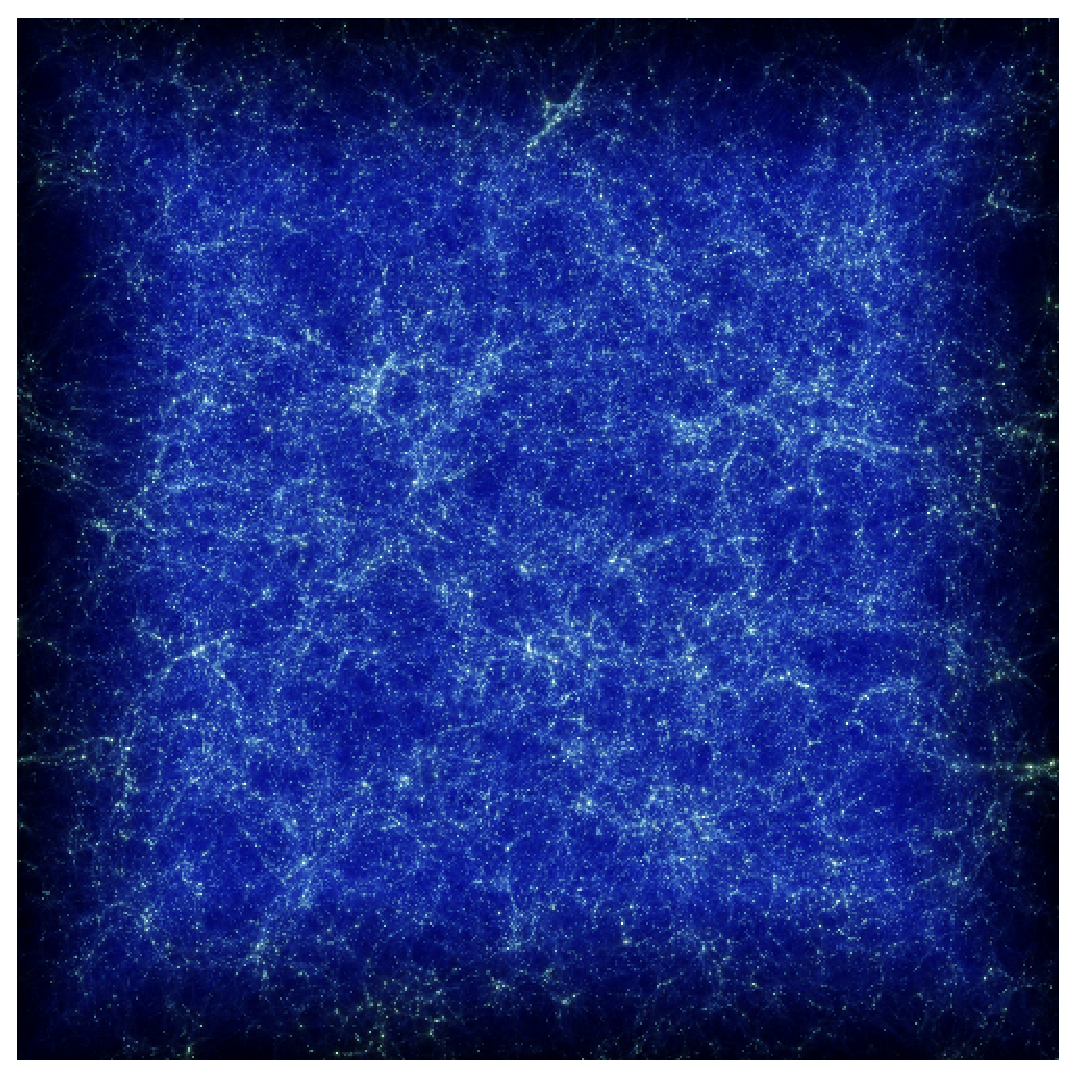
\includegraphics[scale=0.6]{images/box.eps}
\caption{The simulated box, visualized by Splotch. White dots represent stars and galaxies, while the 
diffused blue component is the gas.}
\label{fig:box}
\end{figure}

The dataset adopted in all the tests is the result of a medium sized cosmological 
N-body simulation performed using the Gadget code \cite{gadgeturl}. It consists in about 
400 million particles, with about 200 million of dark matter particles, the same amount 
of baryonic matter (herafter ``gas'') and about 10 million star particles. 
All particles are characterized by their spatial coordinates, velocities
and smoothing length. 
Both the gas and the stars have a number of other quantities associated, that can be used 
as color and intensity. Mass density and temperature for the former, spectral type and age
for the latter. Dark matter is not used in our tests. Figure~\ref{fig:box} shows 
the entire data cube visualized by Splotch.

The large size of the dataset, $\approx 7.5$ GB, can be handled only by a large memory computing node. 
This is not an issue for the GPU, since data are split 
in smaller chunks and loaded iteratively on the accelerator. 

Our tests have all been performed on a 16-core AMD Opteron 6272 2.1 GHz Interlagos processor,
with 32 GBytes of memory, equipped with one NVIDIA Tesla X2090 GPU with 6 GB of GDDR5 memory,
177 GB/sec 
main memory bandwidth, 665 GFlops/sec of peak performance. GCC 4.3.4 and CUDA 5.0.20 
were used for the code compilation.

\subsection{GPU performance tuning}
\label{sec:gpuperf}
In order to get high performance on the GPGPUs, an important aspect is the occupancy (i.e. exploit the underlying architecture as much as possibile trying to avoid that some core is idle during the kernel execution).
From an algorithmic point of view, it is strictly related to the number of threads per block, the number of registers and the size of shared memory used in the kernel because they define the number of resident CUDA blocks (blocks/SM) during the execution. 
Therefore it is important to find a good trade-off among these factors in order to achieve a high occupancy. 

In our implementation, the Rendering kernel is the most critical in this sense. This kernel uses a significat part of the shared memory because each block stores here the Btile and a number $n_p$ of particles to be rendered. 
Hence $n_p$, the tile side $t_x$ (for simplicity we set $t_x=t_y$) and its boundary width $r_0$ are parameters that must be carefully tuned. 
Since $r_0$ is critical both for the particle classification and the CUDA block size, we cannot reduce it as much as we like (we suggest to set $r_0=6$ or $r_0=8$), therefore our tests were focused on finding the best configuration for $n_p$ and $t_x$ which are mainly related to the amount of shared memory used and quite independent of the image resolution. Notice that the tile side is also relevant to the load balancing among different blocks: as the tile side decreases the work load is less unbalanced. However this problem cannot completely overcome when the dataset distribution is heterogenous at all scales. Therefore a further investigation must be done for this issue.

Some possible configurations for these two parameters and the corresponding algorithm performance are presented in Table~\ref{tab:tuning}. In our tests the boundary width and the image resolution are fixed so that the amount of particles processed by the device is always the same. The rendering time includes the computation for all the types of particles (the host contribution is completely overlapped by the device because we have considered a test case were most of the particles are processed by the GPU). Since the tile size affects other computation parts of the code (e.g. particle distribution among tiles), we also consider the total CUDA time as a performance index of the rendering algorithm. 
The necessity to store the Btile and a fixed number of particles in the shared memory for an efficient access to the global memory, do not allow us to reach a full occupancy of the board for the execution of the rendering kernel: the maximum real occupancy obtained is $66.7\%$ both for $n_p = 64$ and $n_p=32$. However the best performance is obtained when $n_p=64$ and $t_x = 12$, which is the configuration used in the following tests.

\begin{table}
\caption{Rendering performance results according to different values of the kernel parameters. We set $r_0=8$ and the resolution $N_{pix}=1024$.}
\begin{center}
\begin{tabular}{|l|l|l|l|l|}
\hline
$n_p$ & $t_x$ (pixels) & Kernel & Rendering & Total CUDA \\
& & Occupancy & Time (sec.) & Time (sec.) \\
\hline
256   & 16 & 0.333 & 9.186 & 16.38 \\
\hline
      & 14 & 0.333 & 7.345  & 15.30 \\
\hline
      & 12 & 0.333 & 6.881  & 14.01 \\
\hline
      & 10 & 0.333 & 6.768 & 14.06 \\
\hline
128   & 16 & 0.333 & 9.159 & 17.00 \\
\hline
      & 14 & 0.333 & 7.302  & 15.30 \\
\hline
      & 12 & 0.5 & 5.074  & 12.08 \\
\hline
      & 10 & 0.5 & 5.016 & 12.30 \\ 
\hline
64    & 16 & 0.5 & 6.516 & 14.23 \\
\hline
      & 14 & 0.5 & 5.387 & 12.55 \\
\hline
      & 12 & 0.667 & 4.423 & 11.34 \\
\hline
      & 10 & 0.667 & 4.393 & 11.45 \\ 
\hline
32    & 12 & 0.667 & 4.515 & 12.41 \\
\hline
      & 10 & 0.667 & 4.483 & 12.43 \\ 
\hline
\end{tabular}
\end{center}
\label{tab:tuning}
\end{table}

\subsection{Performance analysis}
\label{sec:performance}

The main tests' parameters are the data size ($N_{part}$),
the image size ($N_{pix}^2$) and the distribution of the number of pixels 
per particle ($r(p)$) and its expectation value $R_s$.

\medskip
\noindent 
{\bf Scalability with data size}

\noindent
A first series of tests analyze the scalability of the code
with the size of the processed dataset. In these tests, both the image size
and the camera position are kept fixed and set so that all the particles are processed 
by the GPU.

\begin{figure}
\centering
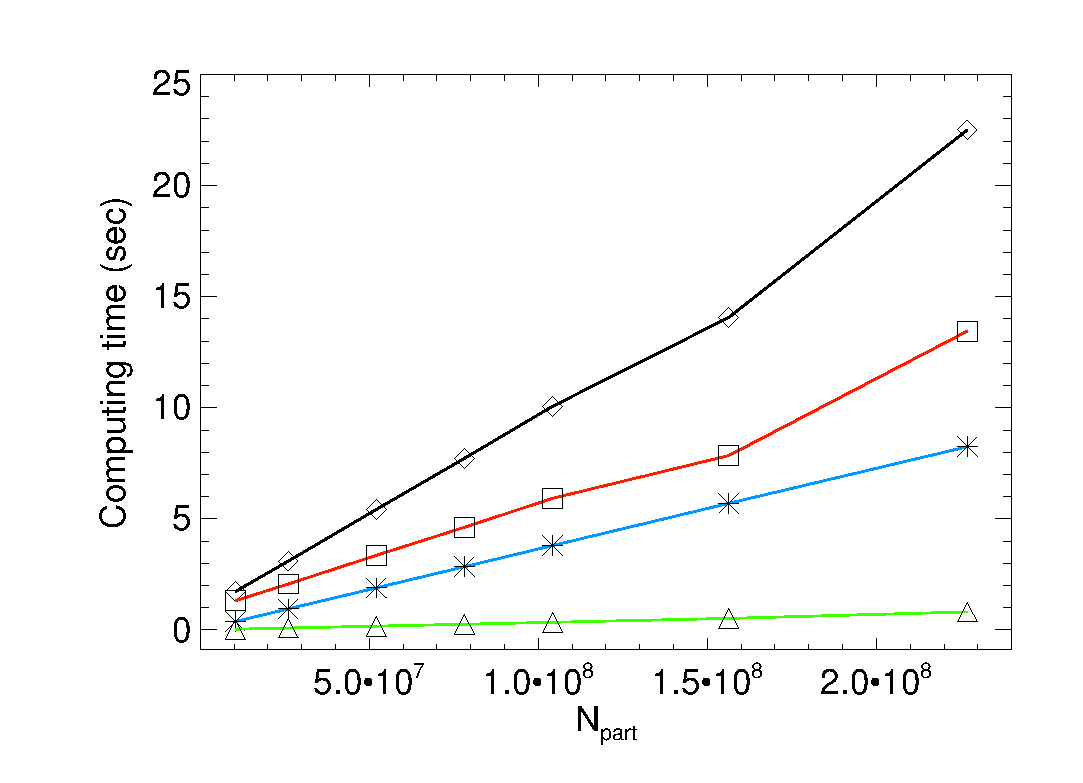
\includegraphics[scale=0.5]{images/scalan.eps}
\caption{Scalability of different Splotch's kernels on the GPU with the dataset size.}
\label{fig:scalability}
\end{figure}

Figure~\ref{fig:scalability} shows different timings, progressively increasing the number of particles
from about $10^7$ up to the total size of about $2.2\times 10^8$. 
The overall computing time scales linearly, 
confirming that the the GPU code preserves the linear dependency from the 
number of particles. 
The Rasterization time always represent 
a minor contribution to the overall time, resulting approximately the 10\% of the rendering 
time. For the original serial implementation, this ratio varies between the 35\% and the 60\%.
This proves that the {\it one-thread-per-particle} approach adopted for this kernel
is extremely effective, making its impact on computing time almost negligible.
The ``Rendering'' time 
is due to the proper rendering kernel. It shows a perfect linear scalability
with $N_{part}$ and represents one of the two main contributions
to the computing time, the other being the sum of the overheads related to all those 
parts specific to the GPU code refactoring 
(e.g. host-device copy time, particle classification etc.). 
This overhead  will be discussed in detail later in this section.

\medskip
\noindent
{\bf Scalability with radii and comparison with the CPU}

\noindent
The smoothing radius depends both on the intrinsic properties of the particle
and from the camera position. 
As discussed in Section~\ref{sec:model} , this has a big impact 
on the implementation of the GPU rendering kernel and
on the performance. In order to investigate the dependency of the performance from
the smoothing radii, we have performed a number of tests 
positioning the camera progressively closer to the dataset center. 
Approaching the center of the 
data cube, the radii distribution moves to larger values. This is expressed 
by the average $R_s$ radius, whose values, for the different cases, are presented in 
Table~\ref{tab:radius}, together with the corresponding number of active particles and computing time. 
Figure~\ref{fig:panorama} shows the images created by Splotch at the different radii.
The image size is kept constant in all the tests, with $N_{pix}$=1000.

\begin{table}
\caption{Average particle radius (left column), number of active particle (center)
and computing time (right column) for seven tests performed varying the average radius.}
\begin{center}
\begin{tabular}{|l|l|l|}
\hline
$R_s$ (pixels) & Active Particles & Time (sec.) \\
\hline
0.30   & 226894837  & 21.12 \\
\hline
0.62   & 225972201  & 22.50 \\
\hline
0.72   & 212746328  & 21.79 \\
\hline
1.40   & 153647633  & 18.88 \\
\hline
3.90   & 64756141   & 25.22 \\
\hline
8.99   & 13686588   & 28.06 \\
\hline
13.66  & 4222214    & 22.15 \\
\hline
\end{tabular}
\end{center}
\label{tab:radius}
\end{table}


\begin{figure}
\centering
\includegraphics[scale=0.2]{images/panorama.eps}
\caption{The particle distribution rendered by Splotch at different camera positions: from very 
far from (top-left image), to very close to the dataset center.}
\label{fig:panorama}
\end{figure}

The same tests have been carried out also with the original Splotch code, in order 
to compare the performance of the two different implementations. 

In the tests the computing time changes according
to the number of active particle, that decreases approaching the center of the particle 
distribution, and the radius $R_s$, that progressively increases. At values of 
$R_s$ larger than unity, a relevant fraction of the particles has radii comparable to the image size
contributing to a large number of pixels, so increasing the computing time 
with the square of their radius. The two opposite trends tend to compensate, keeping  
the computing time between 19 and 28 seconds.

%\begin{figure}
%\centering
%\includegraphics[scale=0.5]{Images/scala-with-R.eps}
%\caption{Scalability of Splotch with the average radius $R_s$}
%\label{fig:Rs}
%\end{figure}

In Figure~\ref{fig:gpucpu}, we present the scalability of the GPU code 
with $R_s$. Since the number of processed particles depends on
the camera position, we use the  
computing time per particle as a meaningful performance
indicator. The curve shows a bi-modal behaviour. For small $R_s$,
the computing time is almost constant, since the performance is dominated
by $N_{part}$ term, which is substantially constant in that range of 
radii. For values of $R_s$ larger 
than unity, the dependency from the square of the radius dominates and the computing time 
rises quickly. 

\begin{figure}
\centering
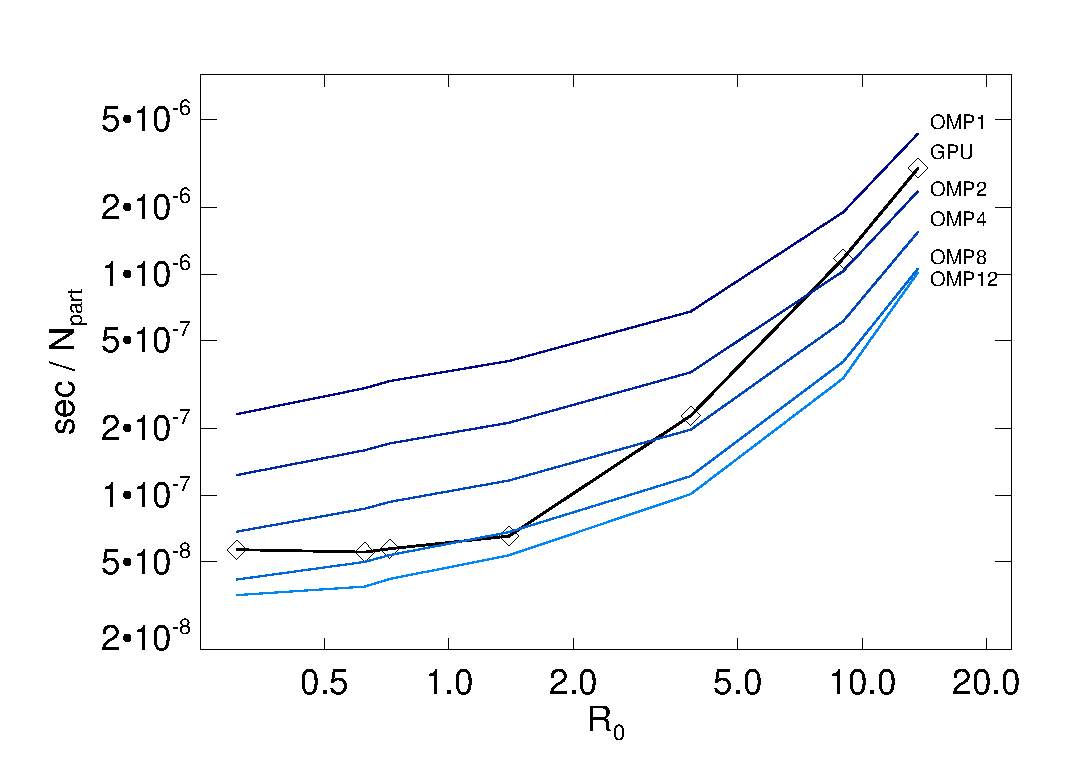
\includegraphics[scale=0.5]{images/scalaomp.eps}
\caption{GPU and CPU performance at different radii. Black line represents the GPU 
computing time, blue lines the CPU times from 16 cores (light blue) to 1 core
(dark blue).}
\label{fig:gpucpu}
\end{figure}

Figure~\ref{fig:gpucpu} presents the comparison between the GPU and the CPU computing time
in the seven cases under investigation, using 
1, 2, 4, 8 and 16 cores, exploiting 
the OpenMP \cite{openmpurl} capability of the original Splotch. As a result all GPU timings can be compared directly to
timings achieved on multi-core and multi-threaded systems, thus giving good indications of non-GPU 
hardware required to achieve performance similar to GPUs. Simply comparing with a single core would not 
be a good indication as parallelized codes do not scale linearly with numbers of processors.

\medskip
\noindent
{\bf GPU timing breakdown}

\begin{figure}
\centering
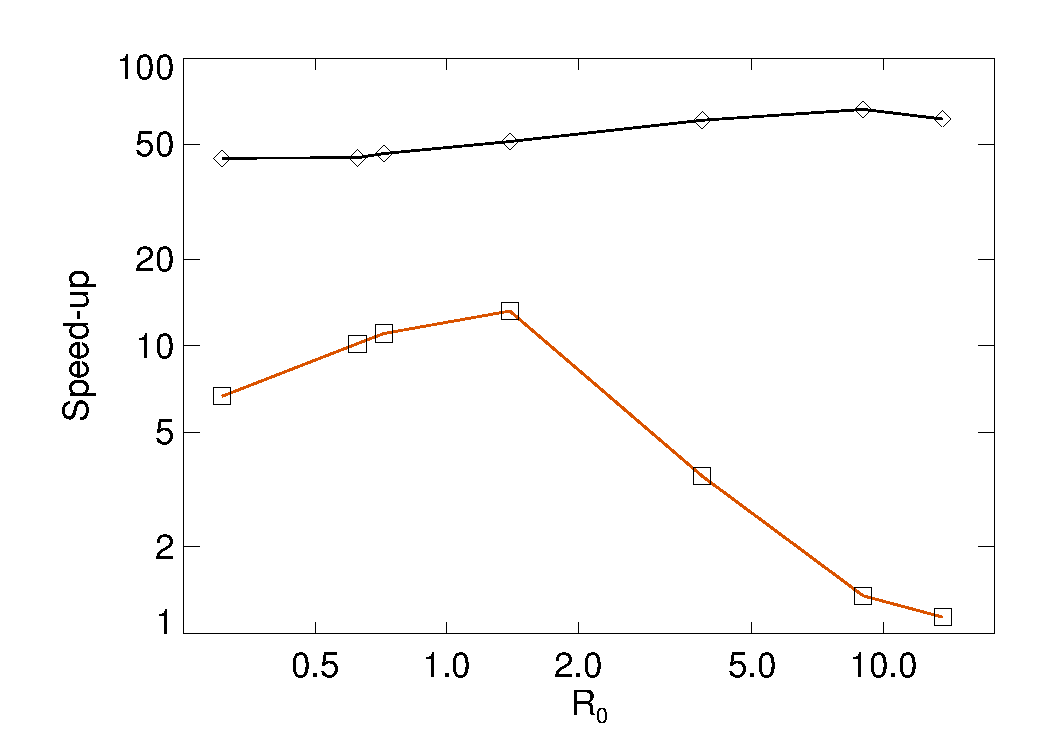
\includegraphics[scale=0.5]{images/speedup.pdf}
\caption{
Speed-up of the Rendering and Rasterization kernels, defined as the ratio
between the time on the GPU and that on the CPU.
}
\label{fig:speedup}
\end{figure}

\begin{figure}
\centering
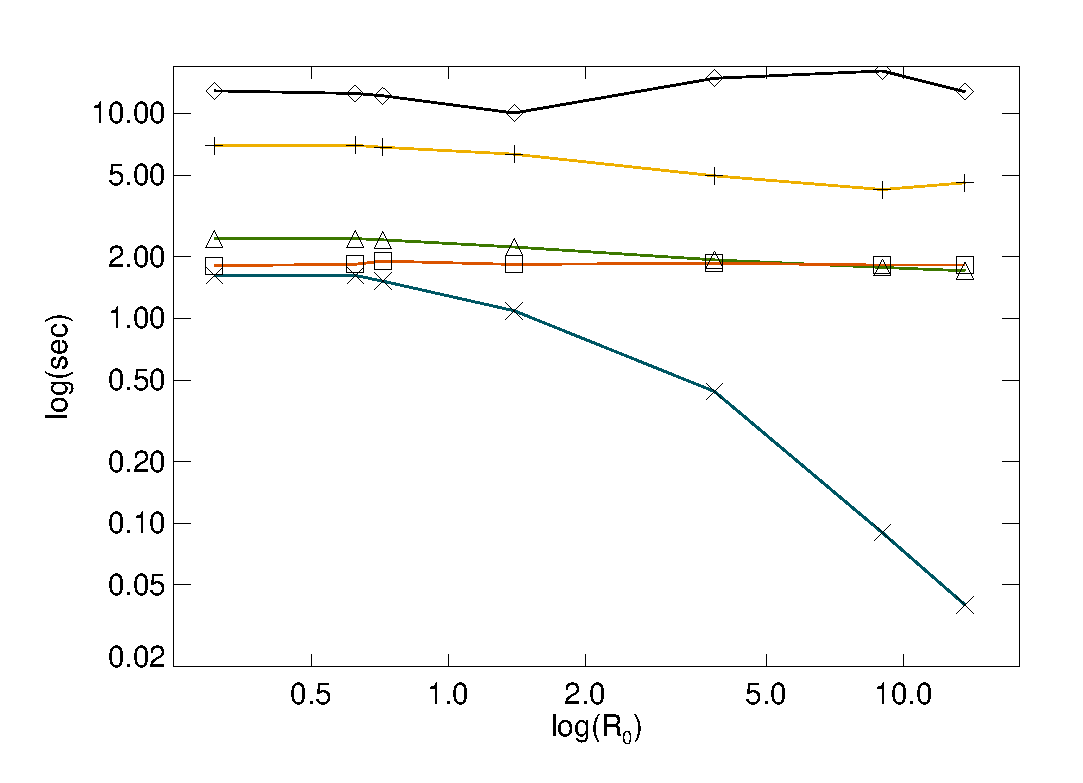
\includegraphics[scale=0.5]{images/over.eps}
\caption{Overhead of the various components implemented for the Splotch's
GPU refactoring. Absolute time is shown on the left image. On the right
the ratio between the time spent in each component and the total GPU 
overhead is shown.}
\label{fig:over}
\end{figure}

\noindent
The same tests presented above, run at different $R_s$, are used also to
analyze the 
time spent in the different kernels. First, we discuss the performance 
achieved by the kernels present also in the original Splotch code: Rasterization and
Rendering.
This is followed by the analysis of the  
{\it GPU overheads}, that is the time spent by functions specific
to the GPU implementation, that are not present in the original code. Such functions can 
be identified as those to offload data to the GPU (Offload),
to setup the GPU environment (Setup),
to sort and reduce data for tiles preparation and memory displacement optimization (Sort),
to remove non active particles and to pack and copy back particles that have to 
be rendered by the CPU (Select) and, finally,
to combine the Btiles in the final image (Image combine).   

In Figure~\ref{fig:speedup} we compare the time needed by the Rasterization and Rendering
kernels on the GPU and the CPU. The speed-up is defined as the ratio between these two
quantities. For the rendering kernel, a maximum speed-up around 13 is obtained for
average radii around the unity. For smaller radii the speed-up tends to decrease due 
to the lower occupancy of the C2 particles rendering kernel which reduce the efficiency of the GPU.
%CLA MARZIA check carefully the previous statement please!!!
As the radius grows, the performance drops, due to the increasing number of particles
processed by the CPU.    

Due to the {\it one-thread-per-particle} approach, the Rasterization kernel is strongly
accelerated by the GPU. The estimated speed-up, ranges between 35 and 25, decreasing 
with larger values of the radius. On the CPU in fact,  
%CLA MARZIA how can you explain this?

Figure~\ref{fig:over} presents the contribution of the different functions
as absolute (left image) and relative (right image) times. This last 
quantity is defined as the time spent by the specific function devided by
the overall GPU overhead. In the right image, also the fraction of the GPU
overhead to the total computing time is shown (xxx line). It is interesting to 
note that this is almost the 50\% of the computing time for small radii,
while it decreases to less than 30\% at large radii, where the
computing time is dominated by the CPU. 

The Image combine time is negligible, accounting for approximately 0.1\% of 
the GPU overhead. This is due mainly to the efficient design of the 
algorithm, which takes full advantage of the multi-thread architecture 
of the accelerator. The Setup and the Selection stages contributes 
almost constant to the overhead. Selection, in particular, 
always accounts for almost the 30\% of the time.
Selection, for particle radii larger than unity, becomes the second 
larger contribution to the overhead. For small radii, the Sort
stage accounts for more than 30\% of the overhead. This is essentially due to 
the large number of particles to be sorted according to their tile index. 
The Sort time drops at larger radii, where more and more particles are
inactive.
 
The most relevant contribution to the GPU overhead is represented by the 
Offload. This is constant, since in all tests all particles are copied 
to the device memory. Hence, it becomes relatively more and more relevant at larger
radii, since the overall GPU overhead decreases. In principle, this Offload overhead could
be strongly reduced adopting CUDA streams and overlapping data copy to 
computation. However, this is currently prevented from the adoption of
Thrust libraries, that, in its current version, does not support asynchronous operations. Furthermore,
in some situations, when the CPU workload is larger than that of
the GPU (e.g. at large radii), such solution would be anyway ineffective.  

\section{Conclusions and Next Steps}
\label{sec:conclusions}

The CUDA implementation of Splotch allows to exploit GPUs 
for the visualization of huge data volumes, such those produced both 
by experiments/observations and by computer simulations. Current trends
in HPC envisage the adoption of accelerators to substantially 
increase the performance of the computing systems, maintaining the power
consumption reasonably low. However, accelerators, and in particular 
GPUs, requires a certain effort to be efficiently exploited, 
supporting only peculiar programming models, that requires codes, or part
of them, to be redesigned and reimplemented before being suitable to such devices. 

Splotch proved to be a challenging application to enable to GPUs. 
In fact, the main computational kernel, the Rendering kernel, poses serious difficulties
to the GPU's programming model, that privileges highly data parallel algorithms.
In order to overcome such difficulties, Splotch's rendering algorithm has been
redesigned with the introduction of specific kernels. These kernels 
introduce an overhead that can be up to the 50\% the overall computing
time. Nevertheless, the final code overperforms the original CPU
version of up to a factor of 4-5, which rises to a factor of 8 when the OpenMP,
multithread parallel version is considered for comparison. Further optimization can
be obtained by the adoption of CUDA streams, overlapping computation 
and data movements. However this is currently prevented by the usage of the 
Thrust libraries, that do not support such kind of operational mode. 
The Splotch GPU code retains also two important features of the original
code: the linear scalability with the number of particles and with the 
image size. 

Although not extraordinary, the attained GPU performance is sufficient 
to run efficiently on the hybrid computing nodes that are more and 
more common in the HPC framework. In order to fully exploit such architectures, 
a further step is necessary, supporting the concurrent usage of 
multiple GPUs, multiple cores and multiple nodes, exploiting respectively the OpenMP and
MPI capabilities of Splotch. This step is expected to pose important 
challenges especially to find the optimal balance in the workload of each of the different 
system components.

\bibliographystyle{plain}
\bibliography{master.bib}	

\end{document}
